\documentclass{standalone}
\usepackage{tikz}
\usetikzlibrary{patterns, positioning}


\begin{document}
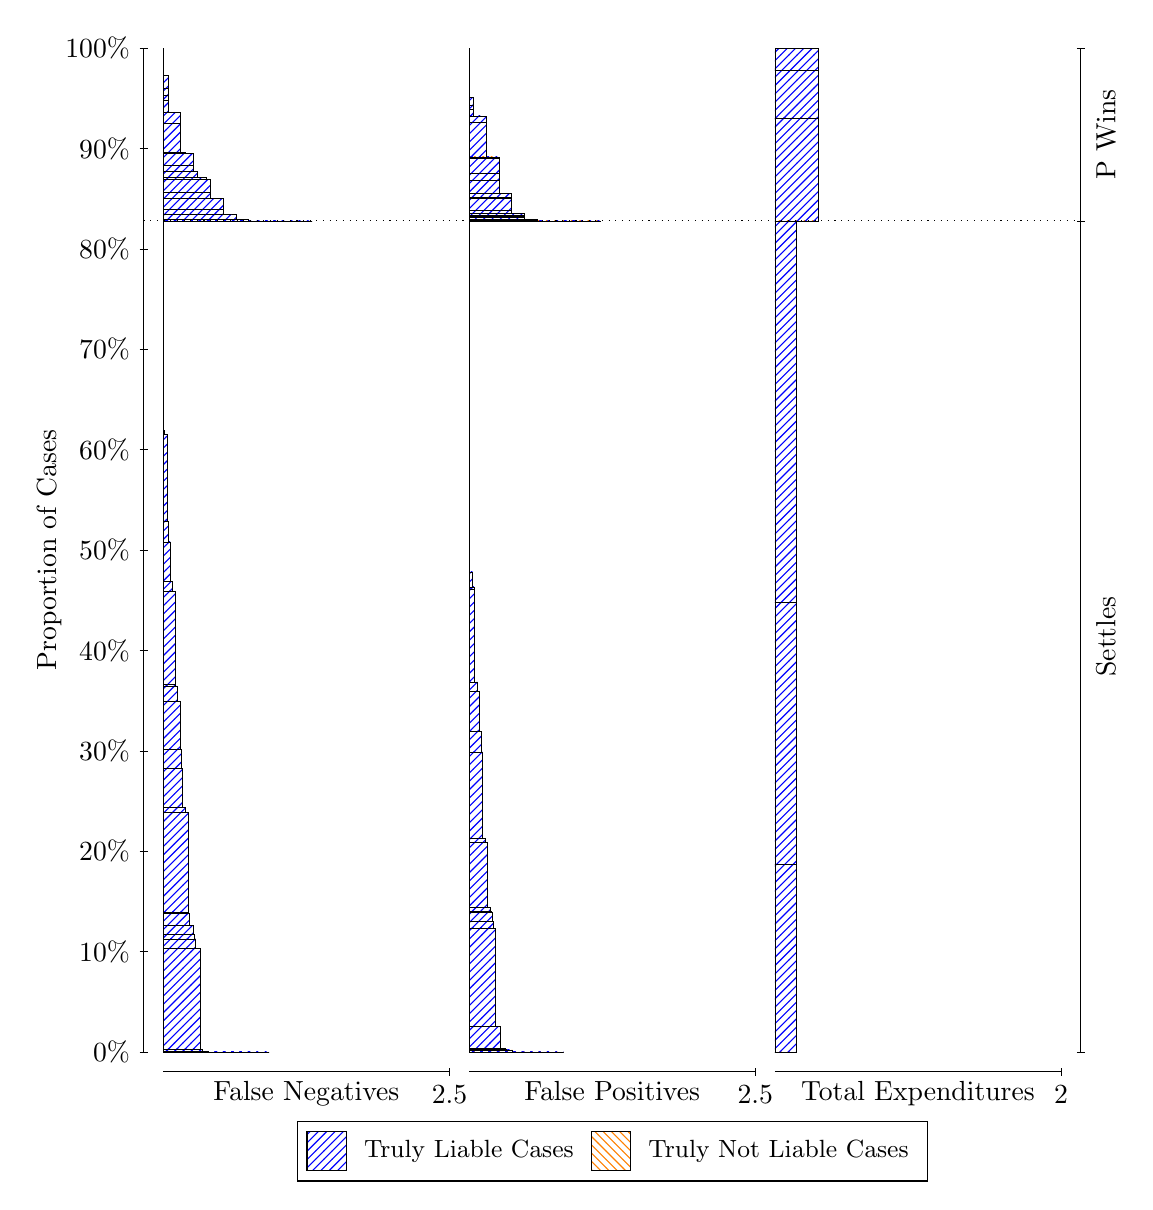
\begin{tikzpicture}
\draw[black, very thin] (1.5,1.75) -- (1.5,14.5);
\node[rotate=90, text=black, anchor=center] at (0.3, 8.125) {Proportion of Cases};
\draw[black, very thin] (1.45,1.75) -- (1.55,1.75);
\node[text=black, anchor=east] at (1.45, 1.75) {0\%};
\draw[black, very thin] (1.45,3.025) -- (1.55,3.025);
\node[text=black, anchor=east] at (1.45, 3.025) {10\%};
\draw[black, very thin] (1.45,4.3) -- (1.55,4.3);
\node[text=black, anchor=east] at (1.45, 4.3) {20\%};
\draw[black, very thin] (1.45,5.575) -- (1.55,5.575);
\node[text=black, anchor=east] at (1.45, 5.575) {30\%};
\draw[black, very thin] (1.45,6.85) -- (1.55,6.85);
\node[text=black, anchor=east] at (1.45, 6.85) {40\%};
\draw[black, very thin] (1.45,8.125) -- (1.55,8.125);
\node[text=black, anchor=east] at (1.45, 8.125) {50\%};
\draw[black, very thin] (1.45,9.4) -- (1.55,9.4);
\node[text=black, anchor=east] at (1.45, 9.4) {60\%};
\draw[black, very thin] (1.45,10.675) -- (1.55,10.675);
\node[text=black, anchor=east] at (1.45, 10.675) {70\%};
\draw[black, very thin] (1.45,11.95) -- (1.55,11.95);
\node[text=black, anchor=east] at (1.45, 11.95) {80\%};
\draw[black, very thin] (1.45,13.225) -- (1.55,13.225);
\node[text=black, anchor=east] at (1.45, 13.225) {90\%};
\draw[black, very thin] (1.45,14.5) -- (1.55,14.5);
\node[text=black, anchor=east] at (1.45, 14.5) {100\%};

\draw[black, very thin] (13.4,1.75) -- (13.4,14.5);
\draw[black, very thin] (13.35,1.75) -- (13.45,1.75);
\node[anchor=west] at (13.35, 1.75) {};
\draw[black, very thin] (13.35,12.305) -- (13.45,12.305);
\node[anchor=west] at (13.35, 12.305) {};
\draw[black, very thin] (13.35,14.5) -- (13.45,14.5);
\node[anchor=west] at (13.35, 14.5) {};

\draw[black, very thin, pattern color=blue, pattern=north east lines] (1.75,1.75) rectangle (3.0943,1.75);
\draw[black, very thin, pattern color=blue, pattern=north east lines] (1.75,1.75) rectangle (2.949,1.75);
\draw[black, very thin, pattern color=blue, pattern=north east lines] (1.75,1.75) rectangle (2.9329,1.75);
\draw[black, very thin, pattern color=blue, pattern=north east lines] (1.75,1.75) rectangle (2.8763,1.75);
\draw[black, very thin, pattern color=blue, pattern=north east lines] (1.75,1.75) rectangle (2.8037,1.75);
\draw[black, very thin, pattern color=blue, pattern=north east lines] (1.75,1.75) rectangle (2.7875,1.75);
\draw[black, very thin, pattern color=blue, pattern=north east lines] (1.75,1.75) rectangle (2.7714,1.75);
\draw[black, very thin, pattern color=blue, pattern=north east lines] (1.75,1.75) rectangle (2.731,1.75);
\draw[black, very thin, pattern color=blue, pattern=north east lines] (1.75,1.75) rectangle (2.7149,1.75);
\draw[black, very thin, pattern color=blue, pattern=north east lines] (1.75,1.75) rectangle (2.6583,1.75);
\draw[black, very thin, pattern color=blue, pattern=north east lines] (1.75,1.75) rectangle (2.6422,1.75);
\draw[black, very thin, pattern color=blue, pattern=north east lines] (1.75,1.75) rectangle (2.626,1.75);
\draw[black, very thin, pattern color=blue, pattern=north east lines] (1.75,1.75) rectangle (2.6099,1.75);
\draw[black, very thin, pattern color=blue, pattern=north east lines] (1.75,1.75) rectangle (2.5695,1.75);
\draw[black, very thin, pattern color=blue, pattern=north east lines] (1.75,1.75) rectangle (2.5534,1.75);
\draw[black, very thin, pattern color=blue, pattern=north east lines] (1.75,1.75) rectangle (2.513,1.75);
\draw[black, very thin, pattern color=blue, pattern=north east lines] (1.75,1.75) rectangle (2.4969,1.75);
\draw[black, very thin, pattern color=blue, pattern=north east lines] (1.75,1.75) rectangle (2.4807,1.7501);
\draw[black, very thin, pattern color=blue, pattern=north east lines] (1.75,1.7501) rectangle (2.4646,1.7501);
\draw[black, very thin, pattern color=blue, pattern=north east lines] (1.75,1.7501) rectangle (2.4484,1.7501);
\draw[black, very thin, pattern color=blue, pattern=north east lines] (1.75,1.7501) rectangle (2.408,1.7506);
\draw[black, very thin, pattern color=blue, pattern=north east lines] (1.75,1.7506) rectangle (2.3919,1.7507);
\draw[black, very thin, pattern color=blue, pattern=north east lines] (1.75,1.7507) rectangle (2.3515,1.751);
\draw[black, very thin, pattern color=blue, pattern=north east lines] (1.75,1.751) rectangle (2.3354,1.751);
\draw[black, very thin, pattern color=blue, pattern=north east lines] (1.75,1.751) rectangle (2.3192,1.7567);
\draw[black, very thin, pattern color=blue, pattern=north east lines] (1.75,1.7567) rectangle (2.3031,1.7591);
\draw[black, very thin, pattern color=blue, pattern=north east lines] (1.75,1.7591) rectangle (2.2869,1.7647);
\draw[black, very thin, pattern color=blue, pattern=north east lines] (1.75,1.7647) rectangle (2.2466,1.7853);
\draw[black, very thin, pattern color=blue, pattern=north east lines] (1.75,1.7853) rectangle (2.2304,1.7883);
\draw[black, very thin, pattern color=blue, pattern=north east lines] (1.75,1.7883) rectangle (2.2223,3.0629);
\draw[black, very thin, pattern color=blue, pattern=north east lines] (1.75,3.0629) rectangle (2.19,3.0703);
\draw[black, very thin, pattern color=blue, pattern=north east lines] (1.75,3.0703) rectangle (2.1739,3.0705);
\draw[black, very thin, pattern color=blue, pattern=north east lines] (1.75,3.0705) rectangle (2.1577,3.1871);
\draw[black, very thin, pattern color=blue, pattern=north east lines] (1.75,3.1871) rectangle (2.1416,3.2403);
\draw[black, very thin, pattern color=blue, pattern=north east lines] (1.75,3.2403) rectangle (2.1254,3.3615);
\draw[black, very thin, pattern color=blue, pattern=north east lines] (1.75,3.3615) rectangle (2.0851,3.5091);
\draw[black, very thin, pattern color=blue, pattern=north east lines] (1.75,3.5091) rectangle (2.0689,3.5297);
\draw[black, very thin, pattern color=blue, pattern=north east lines] (1.75,3.5297) rectangle (2.0609,4.7959);
\draw[black, very thin, pattern color=blue, pattern=north east lines] (1.75,4.7959) rectangle (2.0286,4.8546);
\draw[black, very thin, pattern color=blue, pattern=north east lines] (1.75,4.8546) rectangle (2.0124,4.8571);
\draw[black, very thin, pattern color=blue, pattern=north east lines] (1.75,4.8571) rectangle (1.9963,5.3546);
\draw[black, very thin, pattern color=blue, pattern=north east lines] (1.75,5.3546) rectangle (1.9801,5.6002);
\draw[black, very thin, pattern color=blue, pattern=north east lines] (1.75,5.6002) rectangle (1.964,6.2064);
\draw[black, very thin, pattern color=blue, pattern=north east lines] (1.75,6.2064) rectangle (1.9236,6.399);
\draw[black, very thin, pattern color=blue, pattern=north east lines] (1.75,6.399) rectangle (1.9074,6.4228);
\draw[black, very thin, pattern color=blue, pattern=north east lines] (1.75,6.4228) rectangle (1.8994,7.6047);
\draw[black, very thin, pattern color=blue, pattern=north east lines] (1.75,7.6047) rectangle (1.8671,7.7236);
\draw[black, very thin, pattern color=blue, pattern=north east lines] (1.75,7.7236) rectangle (1.8509,7.7293);
\draw[black, very thin, pattern color=blue, pattern=north east lines] (1.75,7.7293) rectangle (1.8348,8.227);
\draw[black, very thin, pattern color=blue, pattern=north east lines] (1.75,8.227) rectangle (1.8186,8.4945);
\draw[black, very thin, pattern color=blue, pattern=north east lines] (1.75,8.4945) rectangle (1.8025,9.5934);
\draw[black, very thin, pattern color=blue, pattern=north east lines] (1.75,9.5934) rectangle (1.7621,9.6417);
\draw[black, very thin, pattern color=orange, pattern=north west lines] (1.75,9.6417) rectangle (1.75,9.6417);
\draw[black, very thin, pattern color=blue, pattern=north east lines] (1.75,9.6417) rectangle (1.75,12.305);
\draw[black, very thin, pattern color=blue, pattern=north east lines] (1.75,12.305) rectangle (3.6393,12.305);
\draw[black, very thin, pattern color=blue, pattern=north east lines] (1.75,12.305) rectangle (3.4779,12.305);
\draw[black, very thin, pattern color=blue, pattern=north east lines] (1.75,12.305) rectangle (3.3164,12.305);
\draw[black, very thin, pattern color=blue, pattern=north east lines] (1.75,12.305) rectangle (3.1549,12.305);
\draw[black, very thin, pattern color=blue, pattern=north east lines] (1.75,12.305) rectangle (3.1549,12.305);
\draw[black, very thin, pattern color=blue, pattern=north east lines] (1.75,12.305) rectangle (3.0984,12.305);
\draw[black, very thin, pattern color=blue, pattern=north east lines] (1.75,12.305) rectangle (2.9934,12.305);
\draw[black, very thin, pattern color=blue, pattern=north east lines] (1.75,12.305) rectangle (2.9934,12.306);
\draw[black, very thin, pattern color=blue, pattern=north east lines] (1.75,12.306) rectangle (2.9369,12.306);
\draw[black, very thin, pattern color=blue, pattern=north east lines] (1.75,12.306) rectangle (2.8319,12.319);
\draw[black, very thin, pattern color=blue, pattern=north east lines] (1.75,12.319) rectangle (2.7754,12.319);
\draw[black, very thin, pattern color=blue, pattern=north east lines] (1.75,12.319) rectangle (2.7754,12.319);
\draw[black, very thin, pattern color=blue, pattern=north east lines] (1.75,12.319) rectangle (2.6704,12.387);
\draw[black, very thin, pattern color=blue, pattern=north east lines] (1.75,12.387) rectangle (2.6139,12.387);
\draw[black, very thin, pattern color=blue, pattern=north east lines] (1.75,12.387) rectangle (2.509,12.455);
\draw[black, very thin, pattern color=blue, pattern=north east lines] (1.75,12.455) rectangle (2.509,12.594);
\draw[black, very thin, pattern color=blue, pattern=north east lines] (1.75,12.594) rectangle (2.4524,12.594);
\draw[black, very thin, pattern color=blue, pattern=north east lines] (1.75,12.594) rectangle (2.4524,12.595);
\draw[black, very thin, pattern color=blue, pattern=north east lines] (1.75,12.595) rectangle (2.3475,12.666);
\draw[black, very thin, pattern color=blue, pattern=north east lines] (1.75,12.666) rectangle (2.3475,12.833);
\draw[black, very thin, pattern color=blue, pattern=north east lines] (1.75,12.833) rectangle (2.291,12.862);
\draw[black, very thin, pattern color=blue, pattern=north east lines] (1.75,12.862) rectangle (2.186,12.934);
\draw[black, very thin, pattern color=blue, pattern=north east lines] (1.75,12.934) rectangle (2.1295,13.011);
\draw[black, very thin, pattern color=blue, pattern=north east lines] (1.75,13.011) rectangle (2.1295,13.166);
\draw[black, very thin, pattern color=blue, pattern=north east lines] (1.75,13.166) rectangle (2.0245,13.172);
\draw[black, very thin, pattern color=blue, pattern=north east lines] (1.75,13.172) rectangle (1.968,13.54);
\draw[black, very thin, pattern color=blue, pattern=north east lines] (1.75,13.54) rectangle (1.968,13.686);
\draw[black, very thin, pattern color=blue, pattern=north east lines] (1.75,13.686) rectangle (1.863,13.686);
\draw[black, very thin, pattern color=blue, pattern=north east lines] (1.75,13.686) rectangle (1.8065,13.834);
\draw[black, very thin, pattern color=blue, pattern=north east lines] (1.75,13.834) rectangle (1.8065,13.903);
\draw[black, very thin, pattern color=blue, pattern=north east lines] (1.75,13.903) rectangle (1.8065,13.985);
\draw[black, very thin, pattern color=blue, pattern=north east lines] (1.75,13.985) rectangle (1.8065,14.154);
\draw[black, very thin, pattern color=orange, pattern=north west lines] (1.75,14.154) rectangle (1.75,14.154);
\draw[black, very thin, pattern color=blue, pattern=north east lines] (1.75,14.154) rectangle (1.75,14.5);
\draw[black, very thin, pattern color=orange, pattern=north west lines] (5.6333,1.75) rectangle (6.8323,1.75);
\draw[black, very thin, pattern color=blue, pattern=north east lines] (5.6333,1.75) rectangle (6.8323,1.75);
\draw[black, very thin, pattern color=blue, pattern=north east lines] (5.6333,1.75) rectangle (6.6709,1.75);
\draw[black, very thin, pattern color=orange, pattern=north west lines] (5.6333,1.75) rectangle (6.5417,1.75);
\draw[black, very thin, pattern color=blue, pattern=north east lines] (5.6333,1.75) rectangle (6.5417,1.75);
\draw[black, very thin, pattern color=blue, pattern=north east lines] (5.6333,1.75) rectangle (6.5094,1.75);
\draw[black, very thin, pattern color=orange, pattern=north west lines] (5.6333,1.75) rectangle (6.3963,1.75);
\draw[black, very thin, pattern color=blue, pattern=north east lines] (5.6333,1.75) rectangle (6.3963,1.75);
\draw[black, very thin, pattern color=blue, pattern=north east lines] (5.6333,1.75) rectangle (6.3802,1.75);
\draw[black, very thin, pattern color=blue, pattern=north east lines] (5.6333,1.75) rectangle (6.3479,1.7505);
\draw[black, very thin, pattern color=orange, pattern=north west lines] (5.6333,1.7505) rectangle (6.3237,1.7505);
\draw[black, very thin, pattern color=blue, pattern=north east lines] (5.6333,1.7505) rectangle (6.3237,1.7505);
\draw[black, very thin, pattern color=orange, pattern=north west lines] (5.6333,1.7505) rectangle (6.251,1.7505);
\draw[black, very thin, pattern color=blue, pattern=north east lines] (5.6333,1.7505) rectangle (6.251,1.7506);
\draw[black, very thin, pattern color=blue, pattern=north east lines] (5.6333,1.7506) rectangle (6.2349,1.7506);
\draw[black, very thin, pattern color=blue, pattern=north east lines] (5.6333,1.7506) rectangle (6.2187,1.7507);
\draw[black, very thin, pattern color=blue, pattern=north east lines] (5.6333,1.7507) rectangle (6.1864,1.777);
\draw[black, very thin, pattern color=orange, pattern=north west lines] (5.6333,1.777) rectangle (6.1783,1.777);
\draw[black, very thin, pattern color=blue, pattern=north east lines] (5.6333,1.777) rectangle (6.1783,1.777);
\draw[black, very thin, pattern color=blue, pattern=north east lines] (5.6333,1.777) rectangle (6.1622,1.777);
\draw[black, very thin, pattern color=orange, pattern=north west lines] (5.6333,1.777) rectangle (6.1057,1.777);
\draw[black, very thin, pattern color=blue, pattern=north east lines] (5.6333,1.777) rectangle (6.1057,1.7884);
\draw[black, very thin, pattern color=blue, pattern=north east lines] (5.6333,1.7884) rectangle (6.0895,1.7949);
\draw[black, very thin, pattern color=blue, pattern=north east lines] (5.6333,1.7949) rectangle (6.0734,1.7951);
\draw[black, very thin, pattern color=blue, pattern=north east lines] (5.6333,1.7951) rectangle (6.0572,1.8);
\draw[black, very thin, pattern color=blue, pattern=north east lines] (5.6333,1.8) rectangle (6.0249,2.072);
\draw[black, very thin, pattern color=blue, pattern=north east lines] (5.6333,2.072) rectangle (6.0169,2.0723);
\draw[black, very thin, pattern color=blue, pattern=north east lines] (5.6333,2.0723) rectangle (6.0007,2.0746);
\draw[black, very thin, pattern color=orange, pattern=north west lines] (5.6333,2.0746) rectangle (5.9603,2.0746);
\draw[black, very thin, pattern color=blue, pattern=north east lines] (5.6333,2.0746) rectangle (5.9603,3.3268);
\draw[black, very thin, pattern color=blue, pattern=north east lines] (5.6333,3.3268) rectangle (5.9442,3.4113);
\draw[black, very thin, pattern color=blue, pattern=north east lines] (5.6333,3.4113) rectangle (5.928,3.5293);
\draw[black, very thin, pattern color=blue, pattern=north east lines] (5.6333,3.5293) rectangle (5.9119,3.5317);
\draw[black, very thin, pattern color=blue, pattern=north east lines] (5.6333,3.5317) rectangle (5.8957,3.5849);
\draw[black, very thin, pattern color=blue, pattern=north east lines] (5.6333,3.5849) rectangle (5.8634,4.4076);
\draw[black, very thin, pattern color=blue, pattern=north east lines] (5.6333,4.4076) rectangle (5.8554,4.4128);
\draw[black, very thin, pattern color=blue, pattern=north east lines] (5.6333,4.4128) rectangle (5.8392,4.4611);
\draw[black, very thin, pattern color=blue, pattern=north east lines] (5.6333,4.4611) rectangle (5.7989,5.5601);
\draw[black, very thin, pattern color=blue, pattern=north east lines] (5.6333,5.5601) rectangle (5.7827,5.8276);
\draw[black, very thin, pattern color=blue, pattern=north east lines] (5.6333,5.8276) rectangle (5.7666,6.3253);
\draw[black, very thin, pattern color=blue, pattern=north east lines] (5.6333,6.3253) rectangle (5.7504,6.331);
\draw[black, very thin, pattern color=blue, pattern=north east lines] (5.6333,6.331) rectangle (5.7343,6.4499);
\draw[black, very thin, pattern color=blue, pattern=north east lines] (5.6333,6.4499) rectangle (5.702,7.6318);
\draw[black, very thin, pattern color=blue, pattern=north east lines] (5.6333,7.6318) rectangle (5.6939,7.6556);
\draw[black, very thin, pattern color=blue, pattern=north east lines] (5.6333,7.6556) rectangle (5.6777,7.8481);
\draw[black, very thin, pattern color=blue, pattern=north east lines] (5.6333,7.8481) rectangle (5.6374,8.4543);
\draw[black, very thin, pattern color=blue, pattern=north east lines] (5.6333,8.4543) rectangle (5.6333,12.305);
\draw[black, very thin, pattern color=orange, pattern=north west lines] (5.6333,12.305) rectangle (7.3047,12.305);
\draw[black, very thin, pattern color=blue, pattern=north east lines] (5.6333,12.305) rectangle (7.3047,12.305);
\draw[black, very thin, pattern color=orange, pattern=north west lines] (5.6333,12.305) rectangle (7.1432,12.305);
\draw[black, very thin, pattern color=blue, pattern=north east lines] (5.6333,12.305) rectangle (7.1432,12.305);
\draw[black, very thin, pattern color=orange, pattern=north west lines] (5.6333,12.305) rectangle (6.9817,12.305);
\draw[black, very thin, pattern color=blue, pattern=north east lines] (5.6333,12.305) rectangle (6.9817,12.305);
\draw[black, very thin, pattern color=blue, pattern=north east lines] (5.6333,12.305) rectangle (6.9817,12.305);
\draw[black, very thin, pattern color=blue, pattern=north east lines] (5.6333,12.305) rectangle (6.9817,12.305);
\draw[black, very thin, pattern color=orange, pattern=north west lines] (5.6333,12.305) rectangle (6.8202,12.305);
\draw[black, very thin, pattern color=blue, pattern=north east lines] (5.6333,12.305) rectangle (6.8202,12.305);
\draw[black, very thin, pattern color=blue, pattern=north east lines] (5.6333,12.305) rectangle (6.8202,12.305);
\draw[black, very thin, pattern color=orange, pattern=north west lines] (5.6333,12.305) rectangle (6.6587,12.305);
\draw[black, very thin, pattern color=blue, pattern=north east lines] (5.6333,12.305) rectangle (6.6587,12.305);
\draw[black, very thin, pattern color=blue, pattern=north east lines] (5.6333,12.305) rectangle (6.6587,12.306);
\draw[black, very thin, pattern color=blue, pattern=north east lines] (5.6333,12.306) rectangle (6.4973,12.31);
\draw[black, very thin, pattern color=orange, pattern=north west lines] (5.6333,12.31) rectangle (6.4973,12.31);
\draw[black, very thin, pattern color=blue, pattern=north east lines] (5.6333,12.31) rectangle (6.4973,12.312);
\draw[black, very thin, pattern color=blue, pattern=north east lines] (5.6333,12.312) rectangle (6.4973,12.321);
\draw[black, very thin, pattern color=blue, pattern=north east lines] (5.6333,12.321) rectangle (6.3358,12.348);
\draw[black, very thin, pattern color=blue, pattern=north east lines] (5.6333,12.348) rectangle (6.3358,12.365);
\draw[black, very thin, pattern color=orange, pattern=north west lines] (5.6333,12.365) rectangle (6.3358,12.365);
\draw[black, very thin, pattern color=blue, pattern=north east lines] (5.6333,12.365) rectangle (6.3358,12.379);
\draw[black, very thin, pattern color=blue, pattern=north east lines] (5.6333,12.379) rectangle (6.3358,12.403);
\draw[black, very thin, pattern color=orange, pattern=north west lines] (5.6333,12.403) rectangle (6.2793,12.403);
\draw[black, very thin, pattern color=blue, pattern=north east lines] (5.6333,12.403) rectangle (6.2793,12.403);
\draw[black, very thin, pattern color=blue, pattern=north east lines] (5.6333,12.403) rectangle (6.1743,12.44);
\draw[black, very thin, pattern color=orange, pattern=north west lines] (5.6333,12.44) rectangle (6.1743,12.44);
\draw[black, very thin, pattern color=blue, pattern=north east lines] (5.6333,12.44) rectangle (6.1743,12.588);
\draw[black, very thin, pattern color=blue, pattern=north east lines] (5.6333,12.588) rectangle (6.1743,12.599);
\draw[black, very thin, pattern color=blue, pattern=north east lines] (5.6333,12.599) rectangle (6.1743,12.65);
\draw[black, very thin, pattern color=orange, pattern=north west lines] (5.6333,12.65) rectangle (6.1178,12.65);
\draw[black, very thin, pattern color=blue, pattern=north east lines] (5.6333,12.65) rectangle (6.1178,12.65);
\draw[black, very thin, pattern color=blue, pattern=north east lines] (5.6333,12.65) rectangle (6.0128,12.817);
\draw[black, very thin, pattern color=blue, pattern=north east lines] (5.6333,12.817) rectangle (6.0128,12.908);
\draw[black, very thin, pattern color=blue, pattern=north east lines] (5.6333,12.908) rectangle (6.0128,13.1);
\draw[black, very thin, pattern color=blue, pattern=north east lines] (5.6333,13.1) rectangle (6.0128,13.118);
\draw[black, very thin, pattern color=orange, pattern=north west lines] (5.6333,13.118) rectangle (5.9563,13.118);
\draw[black, very thin, pattern color=blue, pattern=north east lines] (5.6333,13.118) rectangle (5.9563,13.118);
\draw[black, very thin, pattern color=blue, pattern=north east lines] (5.6333,13.118) rectangle (5.8513,13.559);
\draw[black, very thin, pattern color=blue, pattern=north east lines] (5.6333,13.559) rectangle (5.8513,13.63);
\draw[black, very thin, pattern color=blue, pattern=north east lines] (5.6333,13.63) rectangle (5.8513,13.633);
\draw[black, very thin, pattern color=orange, pattern=north west lines] (5.6333,13.633) rectangle (5.7948,13.633);
\draw[black, very thin, pattern color=blue, pattern=north east lines] (5.6333,13.633) rectangle (5.7948,13.638);
\draw[black, very thin, pattern color=blue, pattern=north east lines] (5.6333,13.638) rectangle (5.6899,13.719);
\draw[black, very thin, pattern color=blue, pattern=north east lines] (5.6333,13.719) rectangle (5.6899,13.777);
\draw[black, very thin, pattern color=blue, pattern=north east lines] (5.6333,13.777) rectangle (5.6899,13.87);
\draw[black, very thin, pattern color=blue, pattern=north east lines] (5.6333,13.87) rectangle (5.6899,13.87);
\draw[black, very thin, pattern color=orange, pattern=north west lines] (5.6333,13.87) rectangle (5.6333,13.87);
\draw[black, very thin, pattern color=blue, pattern=north east lines] (5.6333,13.87) rectangle (5.6333,14.5);
\draw[black, very thin, pattern color=orange, pattern=north west lines] (9.5167,1.75) rectangle (9.7892,1.75);
\draw[black, very thin, pattern color=blue, pattern=north east lines] (9.5167,1.75) rectangle (9.7892,4.1325);
\draw[black, very thin, pattern color=orange, pattern=north west lines] (9.5167,4.1325) rectangle (9.7892,4.1325);
\draw[black, very thin, pattern color=blue, pattern=north east lines] (9.5167,4.1325) rectangle (9.7892,7.4605);
\draw[black, very thin, pattern color=orange, pattern=north west lines] (9.5167,7.4605) rectangle (9.7892,7.4605);
\draw[black, very thin, pattern color=blue, pattern=north east lines] (9.5167,7.4605) rectangle (9.7892,12.305);
\draw[black, very thin, pattern color=orange, pattern=north west lines] (9.5167,12.305) rectangle (10.062,12.305);
\draw[black, very thin, pattern color=blue, pattern=north east lines] (9.5167,12.305) rectangle (10.062,13.612);
\draw[black, very thin, pattern color=orange, pattern=north west lines] (9.5167,13.612) rectangle (10.062,13.612);
\draw[black, very thin, pattern color=blue, pattern=north east lines] (9.5167,13.612) rectangle (10.062,14.216);
\draw[black, very thin, pattern color=orange, pattern=north west lines] (9.5167,14.216) rectangle (10.062,14.216);
\draw[black, very thin, pattern color=blue, pattern=north east lines] (9.5167,14.216) rectangle (10.062,14.5);
\draw[black, dotted] (1.5,12.305) -- (13.4,12.305);
\draw[black, very thin] (1.75,1.5) -- (5.3833,1.5);
\node[text=black, anchor=north] at (3.5667, 1.5) {False Negatives};
\draw[black, very thin] (5.3833,1.45) -- (5.3833,1.55);
\node[text=black, anchor=north] at (5.3833, 1.45) {2.5};

\draw[black, very thin] (5.6333,1.5) -- (9.2667,1.5);
\node[text=black, anchor=north] at (7.45, 1.5) {False Positives};
\draw[black, very thin] (9.2667,1.45) -- (9.2667,1.55);
\node[text=black, anchor=north] at (9.2667, 1.45) {2.5};

\draw[black, very thin] (9.5167,1.5) -- (13.15,1.5);
\node[text=black, anchor=north] at (11.333, 1.5) {Total Expenditures};
\draw[black, very thin] (13.15,1.45) -- (13.15,1.55);
\node[text=black, anchor=north] at (13.15, 1.45) {2};

\node[text=black, centered, rotate=90] at (13.72, 7.0273) {Settles};
\node[text=black, centered, rotate=90] at (13.72, 13.402) {P Wins};

\draw (7.449999999999999,1.5) node[draw=none] (baseCoordinate) {};
\begin{scope}[align=center]
        \matrix[scale=0.5, draw=black, below=0.5cm of baseCoordinate, nodes={draw}, column sep=0.1cm]{
            \node[rectangle, draw, minimum width=0.5cm, minimum height=0.5cm, pattern color=blue, pattern=north east lines] {}; &
            \node[draw=none, font=\small, text=black] (B) {Truly Liable Cases}; &
            \node[rectangle, draw, minimum width=0.5cm, minimum height=0.5cm, pattern color=orange, pattern=north west lines] {}; &
            \node[draw=none, font=\small, text=black] (B) {Truly Not Liable Cases}; \\
            };
\end{scope}

\end{tikzpicture}
\end{document}